% Body of Section "Learning when to stop copying" (\input from ASRN_Calvario_2026_en.tex).
% Sources: results/citas (CPU, the primary run), results/citas_a100 (its A100 replication),
% docs/TECHNICAL_REPORT.md (Section 7.2). Script: benchmarks/experimento_citas.py.

Copy and MQAR cannot exercise the regulation mechanisms: every evaluated position requires a copy, so retrieval is all
they need, and there the gate, the clock and the Hawkes and streak signals were shown only to be non-intrusive (with
them ASRN copies at 4$\times$ with 99.99\% and 99.98\% in the 2 of 3 seeds that learned and reaches 99.75\% on MQAR
with 4$\times$ the pairs; Section~\ref{sec:ablation}). Their job, deciding whether to copy and when to stop, matters in
free generation, so their active role is tested there, on text whose quotations have a bounded length.

\paragraph{Setup.} The text is random tokens ($V=64$) in which, with probability 0.04 per position, a span of the last
200 tokens of uniform length 6--12 is quoted; in the real text 15.6\% of the tokens are quoted, and runs of
already-seen 4-grams rarely exceed 9 tokens (0.9\% do; the longest is 10). Five models are trained with the same seed,
data and recipe ($d=64$, two local blocks and one ASRN layer, $L=256$, batch 16, learning rate $3\cdot10^{-3}$, 6{,}000
steps on fresh text): the full 1.0 layer; the layer without the Hawkes and streak signals (frozen at their neutral
values); a gate that sees only the hidden state; no gate (fixed at 1); and no clock ($\beta=\alpha=1$, $\gamma=0$). Each
writes 128 tokens after 128-token prompts of 64 validation texts ($T=0.8$ with top-$k=40$ by default, and $T=1$; with
and without prompt-only copy memory). We measure the fraction of written tokens that close an already-seen
4-gram (\emph{quoted}) and the lengths of the runs of such tokens (\emph{streaks}), pooled over seeds 0, 1 and 2. The
primary run is on CPU (\nolinkurl{results/citas/}); the A100 benchmark repeated it (\nolinkurl{results/citas_a100/}).

\begin{figure}[t]
\centering
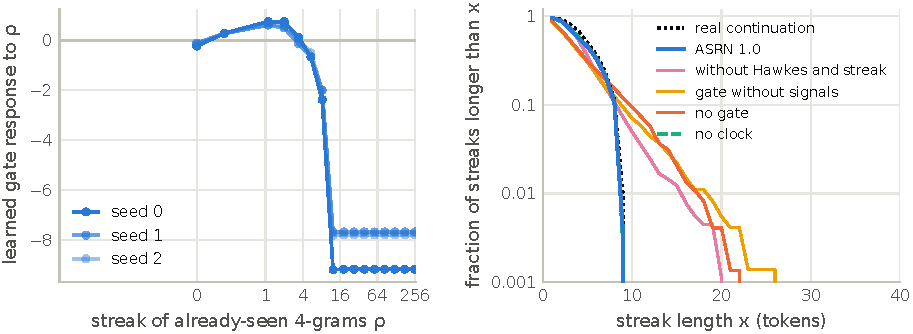
\includegraphics[width=0.94\linewidth]{citas.pdf}
\caption{Bounded-quotation experiment, CPU run. Left: the learned response $f(\rho)$ of the gate of the full layer to
the repetition streak $\rho$, three seeds (symmetric-log axis; nodes equally spaced in $\log(1+\rho)$ up to 256). Right:
fraction of the written streaks longer than $x$ tokens, pooled over the three seeds, with the default sampling
($T=0.8$, top-$k=40$, prompt-only copy memory on); the curve without the clock nearly coincides with the full layer's.}
\label{fig:quote}
\end{figure}

\begin{table}[t]
\centering\small
\setlength{\tabcolsep}{3.3pt}
\begin{tabular}{lrrlrlrl}
\toprule
& \multicolumn{5}{c}{CPU (primary run)} & \multicolumn{2}{c}{A100 replication}\\
\cmidrule(lr){2-6}\cmidrule(lr){7-8}
Text & quoted & mean & max (per seed) & $>9$ & val.\ loss & $>9$ & max (per seed)\\
\midrule
Real continuation & 15.6\% & 5.60 & 10 & 0.9\% & --- & 0.9\% & 10\\
\textbf{ASRN 1.0 (full layer)} & \textbf{20.9\%} & \textbf{5.24} & \textbf{10} (9/10/10) & \textbf{0.3\%} &
3.7027--3.7056 & \textbf{0.3\%} & \textbf{10} (9/10/10)\\
without Hawkes and streak & 19.0\% & 5.22 & 21 (21/20/20) & 7.2\% & 3.7070--3.7079 & 7.9\% & 19 (17/15/19)\\
gate without signals & 13.9\% & 4.69 & 27 (17/23/27) & 9.3\% & 3.7290--3.7586 & 9.2\% & 39 (24/21/39)\\
no gate & 14.7\% & 4.91 & 23 (19/21/23) & 11.8\% & 3.7320--3.7396 & 12.0\% & 21 (21/20/20)\\
no clock & 20.2\% & 5.25 & 10 (10/10/9) & 0.2\% & 3.7042--3.7053 & 0.4\% & 10 (9/10/9)\\
\bottomrule
\end{tabular}
\caption{Writing with the default sampling, seeds 0--2 pooled. \emph{Quoted}: fraction of written tokens that close an
already-seen 4-gram; \emph{mean}, \emph{max}: streak length; $>9$: share of streaks longer than 9 tokens; validation
loss: range over the seeds.}
\label{tab:quote}
\end{table}

\paragraph{What the gate learns.} From the language-modeling loss alone, the full layer's gate learns almost the same
response in the three seeds (Fig.~\ref{fig:quote}, left): a push to copy when a quotation starts ($+0.62$ to $+0.76$ at
$\rho\approx1$), negative by $\rho\approx5$, and a hard brake from $\rho\approx12$ on ($-7.7$ to $-9.2$), flat up to
$\rho=256$: a ``cliff'' just past the longest streak in the data. The response rises and then falls, which a monotone
function of the streak cannot express.

\paragraph{Effect on writing.} With the default sampling the full layer writes streaks like those of the real text
(Table~\ref{tab:quote}, Fig.~\ref{fig:quote}, right): the longest is 10 and 0.3\% exceed 9 tokens. Without the Hawkes
and streak signals the longest streak doubles to 20--21 per seed and 7.2\% exceed 9 tokens, although the model quotes
about as often and its validation loss is only 0.002--0.005 higher: the brake is invisible in the loss and visible only
in what the model writes. With a gate that does not see the signals, or with no gate, the model quotes less, still
cannot stop, and its validation loss worsens by 0.03--0.05; without the clock it writes like the full layer. The
ordering holds in every sampling condition (longest streak per seed 9--10 for the full layer, up to 11 with the
quotation-preserving temperature off, against 15--36 for the three variants), and at $T=0.8$ turning that temperature
off raises the quoted fraction from 20.9\% to 27.6\% and the streaks above 9 tokens from 0.3\% to 2.8\%.

\paragraph{Replication on the A100.} The same 5 variants, 3 seeds and 6{,}000 steps on the GPU reproduce the result
(Table~\ref{tab:quote}, right): across all sampling conditions the full layer's longest streak per seed is 9--12 (12
only with prompt-only copy memory off at $T=0.8$) and without the clock 9--10, against 14--24 without Hawkes and streak,
15--39 with a gate without signals and 18--31 without a gate. The validation loss is 0.001--0.004 higher without Hawkes
and streak and 0.025--0.045 higher with a gate without signals or no gate, and the gate response has the same shape
($+0.64$ to $+0.75$ at $\rho\approx1.1$, $-7.65$ to $-8.41$ from $\rho\approx12.3$ on).

\paragraph{Scope.} This is one synthetic task with three seeds, $d=64$ and one ASRN layer. It removes the Hawkes and
streak signals together and the gate's inputs as a whole, so it validates the gate and its repetition signals, not each
signal separately. The clock has no measurable effect here, as expected for a task without topic shifts. How often a
quotation \emph{starts} is not calibrated (the quotation-preserving temperature covers only its continuation): the full
layer quotes 20.9--22.2\% of the tokens at $T=0.8$ and 9.3--11.2\% at $T=1$ (21.8--24.2\% and 10.1--11.8\% on the
A100), against 15.6\% in the real text.
